\label{chapter:problems}

Writing Multithreaded programs can encounter concurrency errors and performance anomalies. This thesis discusses in detail of two different categories of problems, including false sharing and non-deterministic executions. They belongs to performance problems and reliable problems. We discuss the definitions, causes of these problems and their possible consequence as follows.

\section{False Sharing}

\subsection{False Sharing and True Sharing}
% What is the definition of false sharing?
False sharing occurs when different processors in a shared-memory parallel system are referencing different fields within the same coherence block (page or cache line) simultaneously, thereby inducing ``unnecessary'' coherence operations~\cite{Bolosky:1993:FSE:1295480.1295483}. 

Although it is difficult or impossible to know where a thread runs in an actual execution, we can conservatively assume that different threads run on different processors with separate cache. Thus, in the multithreaded environment, false sharing simply implies: two threads access two different words of the same cache line, while one of them is a write operation. False sharing is shown in Figure~\ref{fig:fs}. 
Based on the relationship of false sharing objects, 
false sharing can be classified into inter-object and intra-object false sharing. When two different objects in the same cache line are accessed by different threads simultaneously, that is inter-object false sharing. Otherwise, it is intra-object false sharing. 

There is another concept, true sharing, which is opposite of false sharing. In true sharing (Figure~\ref{fig:ts}), multiple threads are accessing the same word. 

\begin{figure*}
\begin{center} 
\subfigure[False sharing]{%
   \label{fig:fs}
   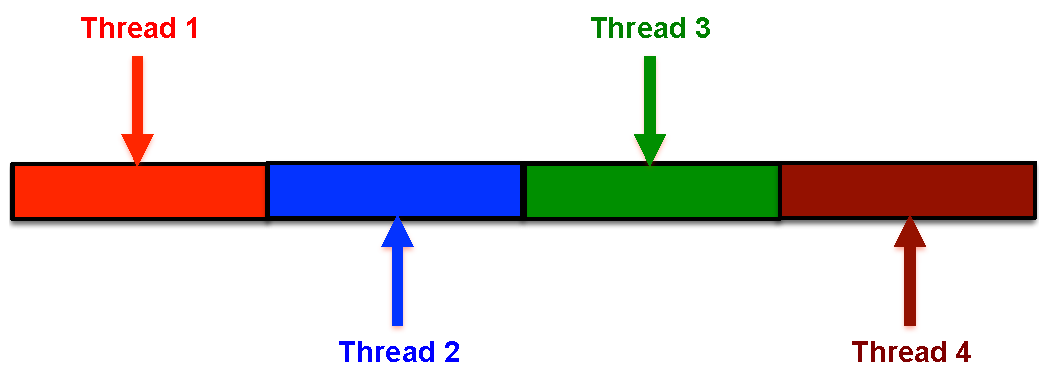
\includegraphics[width=2.4in]{sheriff/figure/falsesharing.pdf}
}%
\hspace{50pt}
\subfigure[True sharing]{%
   \label{fig:ts}
   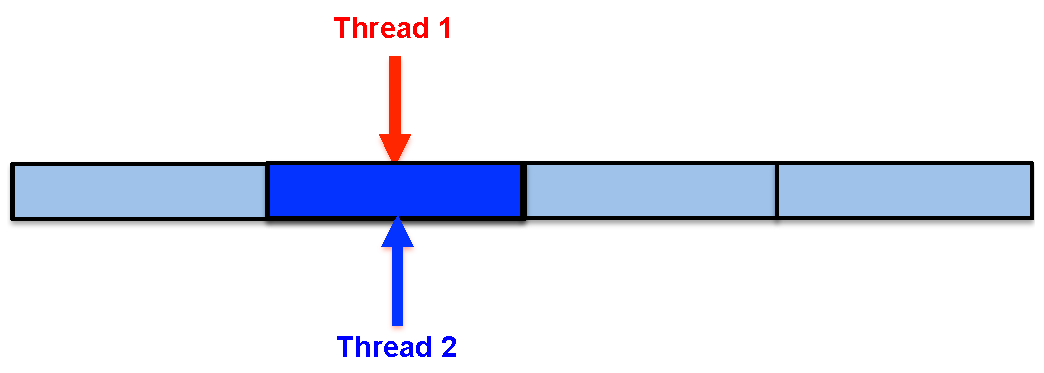
\includegraphics[width=2.4in]{sheriff/figure/truesharing.pdf}
}%
\end{center}
%\includegraphics{fig/potential.pdf}
\caption{False sharing and true sharing in a cache line with 4 words. }
\label{fig:fsexample}
\end{figure*}

% The classification of false sharing?

\subsection{Reason of False Sharing}

As shown in Figure~\ref{fig:fsexample}, false sharing only occurs when the size of coherence block is larger than that of a single word. Multiple processors may reference different words of the same coherence block. In this perspective, a single-word block size can avoid false sharing problems. 

However, this is not the actual case. In reality, the size of coherence block (cache line) is normally 32 or 64 bytes. The reason of using multiple words is to reduce the groups of transfers between the main memory and the cache since programs always have some spatial locality of reference. Those adjacent words are very likely to be referenced in the future.

From the performance perspective, reducing the block size to one word may minimize the data to transferred, but can increase the number of transfers. Thus, the overhead of transferring less data at a time can be larger than the benefit of eliminating false sharing coherence traffic. Actually, the hardware trend of increasing the size of cache line makes false sharing problems increasingly common. 

\subsection{Performance Impact}
\label{falsesharing}
False sharing can greatly slow down the execution of multithreaded programs, which depends on many factors, including block size, data layout, program access patterns, and the cost of coherence operations~\cite{Bolosky:1993:FSE:1295480.1295483}. 

In a typical shared-memory system, each processor may has a separate cache. In order to increase the access speed, when a processor references a word, the data of the same cache line is fetched from the main memory to its corresponding cache. 
When multiple processors are accessing different words of the same cache line, shared data can be replicated into caches of processors that access them. Thus, it is very important to maintain the coherence across different processors: 
if any copy has been changed, this change should be propagated to other processors immediately for correctness reason. This also means that duplicates in other processors must be invalidated at first. This propagation is very time-consuming, because it wastes CPU time and memory bandwidth simultaneously. 

However, in the false sharing case, this propagation is not necessary because different threads are not actually shared the same data. 
When there are interleaved writes (by different processors) on the same cache line, the ping-pong effect of 
loading-and-invalidating of data on this cache line can  
greately slow the execution of programs
because the speed to load data from the main memory is much slower than that to access cache directly
(about 20 $\times$ slower). 
Programs with false sharing can even run slower in a multi-core machine 
than in a single-core machine, losing the benefit of multiple cores.  


% at first 
%in the unit of a cache line (64 or 128 bytes normally).  
%In the false sharing situation, because different threads are accessing 
%different words in the same cache line and one of those accesses is a write.
%When a write access is happening, other copies in other caches of this cache line 
%needs to be invalidated to ensure the correctness. 


Many common programming practices can easily cause false sharing. For example, different threads accessing different entries of the same global array, listed in Figure~\ref{fig:falsesharingexample}, is such an example. This example is a toy program, which different threads are cooperating to increment a global array. This example has no correctness problem, but with a serious performance problems. 

\begin{figure*}[!ht]
{\centering
\fbox{
\subfigure{\lstinputlisting[numbers=none,frame=none,boxpos=t]{fig/falsesharing.sample1}}
\hspace{20pt}
\subfigure{\lstinputlisting[numbers=none,frame=none,boxpos=t]{fig/falsesharing.sample2}}
}
\caption{False sharing problem
\label{fig:falsesharingexample}}
}
\end{figure*}

We actually run this program on a real machine with 8 cores. We specifically choose different number of threads, from 1 thread to 8 threads, to finish the same task. 
Performance results can be seen in Figure~\ref{fig:fsperfimpact}. We specifically disable hardware cores to match the number of threads. We can see that false sharing can greatly impact the performance, which causes huge difference between the actual performance and the expected performance. We also notice that the performance is even worse when there are more threads and cores. 

\begin{figure*}[!t]
\centering
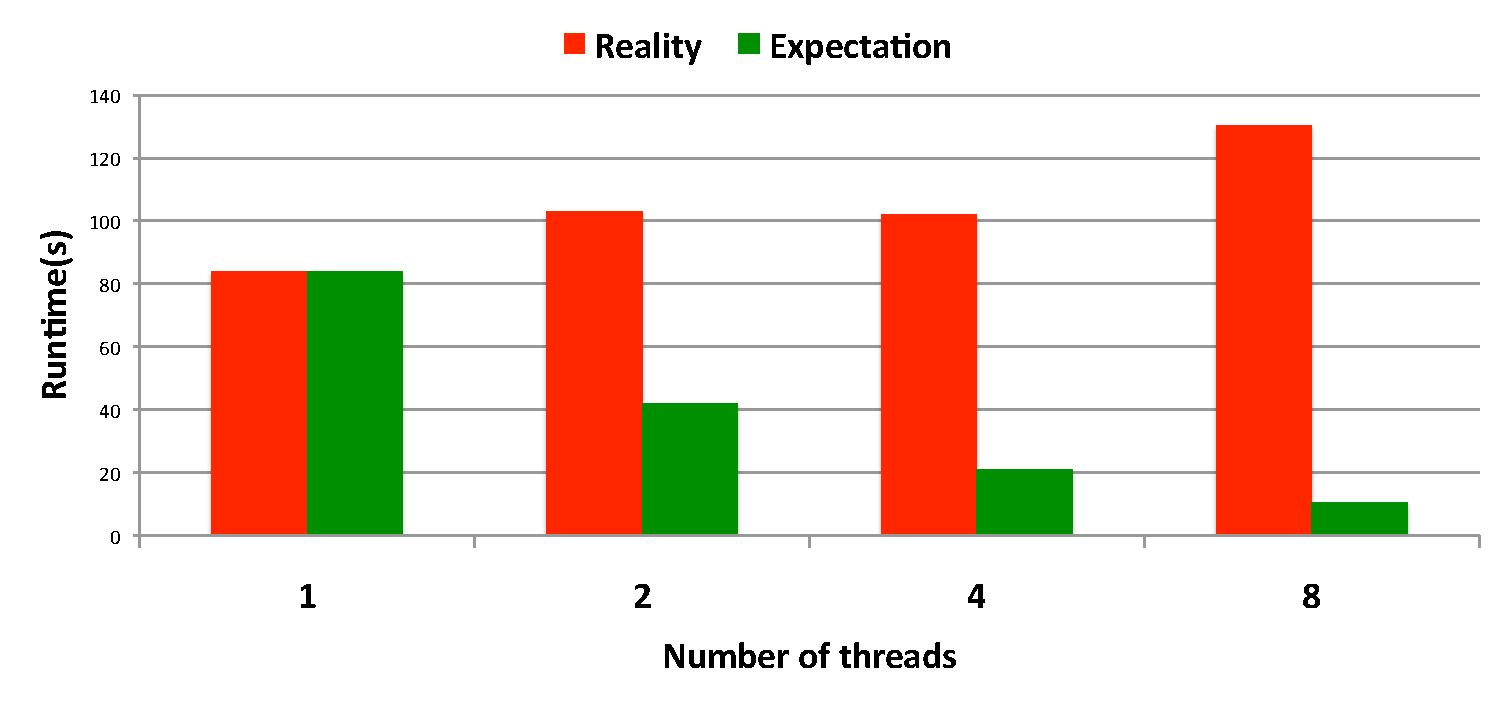
\includegraphics[width=5in]{fig/fsperfimpact.pdf}
\caption{
False sharing performance impact for the simple program shown in Figure~\ref{fig:falsesharingexample}.
\label{fig:fsperfimpact}
}
\end{figure*}

\subsection{Fixing False Sharing}
There are several ways to fix false sharing related problems after they are found. The basic idea is to prevent multiple threads accessing the same cache line simultaneously.  

The first way is to change the size of corresponding structure or class. One example of this can be seen in Section~\ref{sec:fsfixexample}.

The second way is to use some thread-local variable to replace those shared variable.
The problem shown in Figure~\ref{fig:falsesharingexample} can be fixed using this way. It is shown in Figure~\ref{fig:falsesharingexamplefix}. 

\begin{figure*}[!ht]
{\centering
\fbox{
\subfigure{\lstinputlisting[numbers=none,frame=none,boxpos=t]{fig/falsesharing.sample2fix}}
}
\caption{Fixing the false sharing problem shown in Figure~\ref{fig:falsesharingexample}.
\label{fig:falsesharingexamplefix}}
}
\end{figure*}

There also existing several approaches to fix false sharing problems automatically, described in detail in Section~\ref{sec:fspreventwork}. However, they all suffer different shortcomings. 


%are accessing we can use the padding or thread-local variable to   
% why it is important
% why it can cause the performance problem
% one or two example of false sharing problem

% how to fix this kindd of problem: padding, 

\section{Non-determinism}

\subsection{Definition}

\subsubsection{Program Input}
A program with the same input does not always create the same output in different executions,
known as ``non-determinism'' problem.
Executions of multithreaded programs are full of non-determinism: 
thread schedulings, memory access on shared data, operations depending on timing 
and non-deterministic synchronizations can easily cause different behavior of the same program.
A simple example can be seen in Figure~\ref{fig:nondeterminism}.

\subsubsection{Program Output}

\begin{figure*}[!ht]
{\centering
\fbox{
\subfigure{\lstinputlisting[numbers=none,frame=none,boxpos=t]{fig/nondeter.sample1}}
\hspace{12pt}
\subfigure{\lstinputlisting[numbers=none,frame=none,boxpos=t]{fig/nondeter.sample2}}
\hspace{12pt}
\subfigure{\lstinputlisting[numbers=none,frame=none,boxpos=t]{fig/nondeter.sample3}}
}
\caption{Non-determinism problem 
\label{fig:nondeterminism}}
}
\end{figure*}

\subsection{Reason of Non-determinism}

\label{sec:nondeterminism}
This program with \pthreads{} can print ``1,0'', ``0,1'' or ``1,1'' in the end, 
depending on the order of memory accesses from different threads. 
About 99.43\% it will print ``1,0'', while 0.56\% it will print ``0,1''
and 0.01\% it will print ``1,1''.
For this case, unexpected results caused by race condition are rare (about 0.01\%). 
It is unlikely to detect race conditions in the development phase. 
So this non-determinism problem can be easily leaked to users.
Users can observe errorneous results that are not discovered in testings. 
Even worse, these errors may not be reproducible by the development team using
a different hardware configuration. 

\subsection{Effect of Non-determinism}

Deterministic execution is a nice property: programs always produce 
the same output given the same input.
Determinism greatly simplifies the understanding and debugging of multithreaded programs.

\subsection{What is the target of determinism}
\subsection{What kind of guarantee}
